\documentclass{article}

\usepackage[french]{babel}
\usepackage[utf8]{inputenc}
\usepackage[T1]{fontenc}

\usepackage{xcolor}
\usepackage{amsmath}
\usepackage{amssymb}
\usepackage{amsfonts}
\usepackage{graphicx}
\usepackage{caption}
\usepackage{float}
\usepackage{dcolumn}
\usepackage{textcomp}

\newcolumntype{d}[1]{D{.}{.}{#1}}
%%%%%%%%%%%%%%%% Lengths %%%%%%%%%%%%%%%%
\setlength{\textwidth}{15.5cm}
\setlength{\evensidemargin}{0.5cm}
\setlength{\oddsidemargin}{0.5cm}

%%%%%%%%%%%%%%%% Variables %%%%%%%%%%%%%%%%
\def\projet{1}
\def\titre{Méthodes de calcul numérique / Limites de la machine }
\def\groupe{2}
\def\equipe{1}
\def\responsible{tmichel003}
\def\secretary{alamhamdi001}
\def\others{kdieu, matguedon, mkasour}

\begin{document}

%%%%%%%%%%%%%%%% Header %%%%%%%%%%%%%%%%
\noindent\begin{minipage}{0.98\textwidth}
  \vskip 0mm
  \noindent
  { \begin{tabular}{p{7.5cm}}
      {\bfseries \sffamily
        Projet n$^{\circ}$\projet} \\
      {\itshape \titre}
    \end{tabular}}
  \hfill 
  \fbox{\begin{tabular}{l}
      {~\hfill \bfseries \sffamily Groupe n$^{\circ}$\groupe\ - Équipe n$^{\circ}$\equipe
        \hfill~} \\[2mm] 
      Responsable : \responsible \\
      Secrétaire : \secretary \\
      Codeurs : \others
    \end{tabular}}
  \vskip 4mm ~

  ~~~\parbox{0.95\textwidth}{\small \textit{Résumé~:} \sffamily Ce projet consiste à évaluer les problèmes qui peuvent apparaître lors de l’utilisation d’opérations élémentaires, voire d’algorithmes plus poussés, sur des nombres flottants. La première partie s’intéresse à trouver des exemples dans lesquels les opérations élémentaires sont insuffisamment précises. La seconde partie donne des exemples d’algorithmes utilisés dans des conditions de calcul en basse précision.}
   \vskip 1mm ~

\end{minipage}

%%%%%%%%%%%%%%%% Main part %%%%%%%%%%%%%%%%
\section{Représentation des nombres en machine}

\begin{enumerate}
    \item 
    Le but de cet exercice était de créer une fonction qui calcule la représentation décimale réduite d'un nombre x pour une précision p. Nous allons présenter l'algorithme réalisé sous forme d'étapes.
     
    \paragraph{Etape 1}
    Tout d’abord, on transforme le nombre d'origine de manière à ce que sa valeur soit comprise entre 0 et 1 exclus et que son premier chiffre des décimales soit strictement supérieur à 0. On retiendra le nombre d’opérations nécessaires pour obtenir ce résultat dans une variable nommée n.
    
    \paragraph{Etape 2}
    Puis, on effectue une nouvelle opération pour obtenir une partie entière dont la taille correspond à la précision p demandée. Pour cela on multiplie le nombre obtenu précédemment par $10^p$.
    
    \paragraph{Etape 3}
    Ensuite, on réalise un arrondi sur le chiffre des unités et on ne récupère que la partie entière.
    
    \paragraph{Etape 4}
    Enfin, on effectue une dernière multiplication sur le nombre obtenu pour revenir au format d’origine du nombre :
    \begin{itemize}
        \item Si le nombre d’origine est inférieur à 1 : on multiplie par $10^{n-p}$
        \item Sinon : on multiplie par $10^{1-n-p}$
    \end{itemize}
    
    \paragraph{}
    \textit{Pour présenter les opérations effectuées, deux exemples sont dévelopés en Figure~\ref{exemple_1} pour une précision p = 6. On voit que, pour la première étape, des divisions sont nécessaires (n=6 divisions par 10) sur le premier exemple tandis que des multiplications (n=3 multiplications par 10) sont effectuées sur le deuxième.}
    
    \begin{figure}[H]
        \centering
        \begin{tabular}{ | d{10} | l | l | l | d{9} | }
            \hline	
            \textbf{Exemples} & \textbf{Etape 1} &  \textbf{Etape 2} & \textbf{Etape 3} & \textbf{Etape 4} \\ \hline
            10507.1823 & 0.105071823 & 105071.823 & 105072 & 10507.2\\ \hline	
            0.0001857563 & 0.1857563 &  185756.3 & 185756 & 0.000185756\\
            \hline	
        \end{tabular}
        \caption{Deux exemples pour une précision de 6}  
        \label{exemple_1}
    \end{figure}
    
    \paragraph{}
    Avec cet algorithme, nous obtenons les mêmes résultats que dans les exemples du sujet sauf pour le nombre $\pi$ à la précision 6 où nous obtenons 3.1415900000000003. Cela est dû à la représentation des nombres décimaux par un ordinateur. Ce phénomène est évoqué brièvement dans la deuxième partie de ce rapport.
    \newline
        
    Nous avions d'abord un algorithme qui calculait l'arrondi en manipulant des chaînes de caractères et nous obtenions les bons résultats mais il était demandé de ne pas passer par des chaînes de caractères.
    
    \item Pour l'addition de deux nombres x et y, en représentation décimale réduite (RDR) à une précision p, la fonction \texttt{add\_rp(x, y, p)} retourne la somme de RDR de x et de y à la précision p. Pour la multiplication, la fonction \texttt{mul\_rp(x, y, p)} renvoie le produit de RDR de x et de y à la précision p.
    
    \item Les deux fonctions \texttt{relative\_err\_add(x, y, p)} et \texttt{relative\_err\_mul(x, y, p)} calculent l'erreur relative pour la somme et la multiplication de x et y à la précision p. 
    
    \item Pour observer l'erreur relative maximale de l'addition et de la multiplication, nous avons choisi de regarder le résultat des deux fonctions précédentes pour x = $\pi$ car il a un nombre infini de décimales. Par ailleurs, nous avons pris une précision de 1 car plus la précision est petite, plus l'erreur relative est élevée. Enfin, nous avons fait varier y sur l'intervalle [0,100] pour l'addition et [1,100] pour la multiplication.
    \newline
    
    Que ce soit sur l'addition (Figure \ref{repr_err_rel_add_1}) ou la multiplication (Figure \ref{repr_err_rel_mul_1}), on observe que l'erreur relative maximale est supérieure à 0.30 pour l'addition et à 0.35 pour la multiplication. Cela est confirmé par le calcul de la valeur maximale précise en Figure \ref{max_err_rel} où l'on voit que l'erreur relative de la somme est d'environ 0.32 et celle de la multiplication est d'environ 0.36. Nous avons donc une erreur relative maximale de plus de 30\% ce qui est plutôt élevée.
    
    \begin{figure}[H]
       \begin{minipage}{0.5\textwidth}
            \centering
            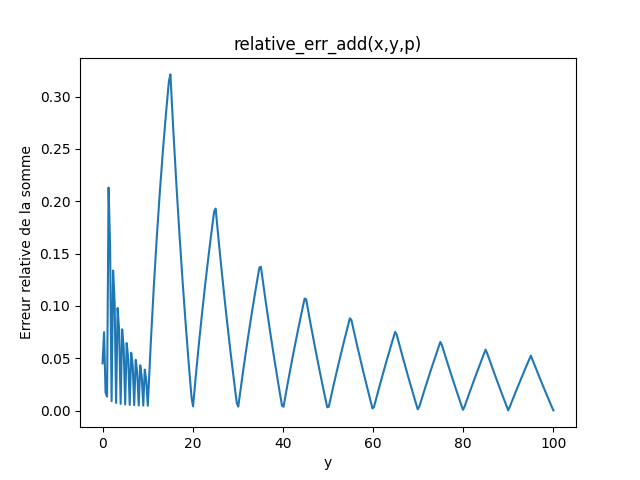
\includegraphics[width=1.1\linewidth]{images/relative_err_add_p1.png}
            \caption{Erreur relative pour l'addition}
            \label{repr_err_rel_add_1}
        \end{minipage}\hfill
        \begin{minipage}{0.5\textwidth}
            \centering
            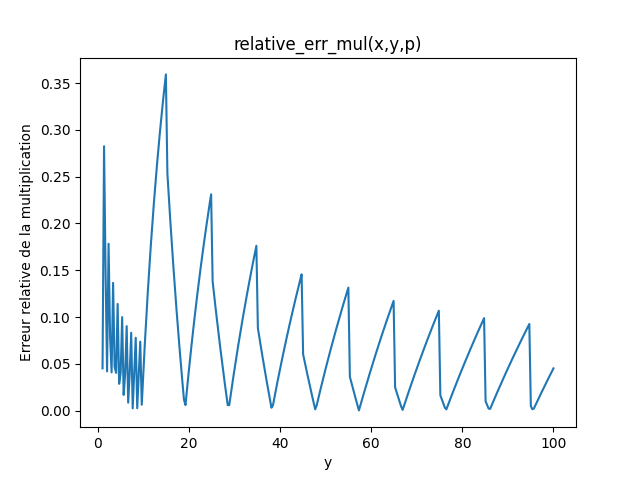
\includegraphics[width=1.1\linewidth]{images/relative_err_mul_p1.png}
            \caption{Erreur relative pour la multiplication}
            \label{repr_err_rel_mul_1}
       \end{minipage}\hfill
    \end{figure}
    
    \begin{figure}[H]
        \centering
        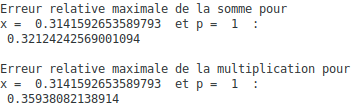
\includegraphics[width=0.5\linewidth]{images/max_err_p1.PNG}
        \caption{Erreur relative maximale pour l'addition et la multiplication}
        \label{max_err_rel}
    \end{figure}
        
        
    
    \item Pour calculer nous même une valeur approchée de log(2) à la précision p, nous effectuons la somme \eqref{log_2} en incrémentant n tant que l'erreur relative est supérieure à $10^{-p}$. Nous avons donc, en parrallèle, un calcul de l'erreur relative qui s'inspire de celui de l'addition : \\ $|log(2) - rp(res, p)| / log(2)$ où res est le résultat courant de la somme.
    
    \begin{equation}
        \label{log_2}
        log(2) = \sum_{n=1}^{\infty} \frac{(-1)^{n+1}}{n}
    \end{equation}
    
\end{enumerate}


\section{Algorithmes CORDIC}
\begin{enumerate}
    \item 
    L'algorithme CORDIC (pour COordinate Rotation DIgital Computer, « calcul numérique par rotation de coordonnées ») est un algorithme créé en 1957 par un ingénieur américain, Jack Volder, et qui permet de calculer des valeurs approchées des fonctions trigonométriques. Cet algorithme a notamment été utilisé sur les premières calculatrices, au vu des rescources limitées à notre disposition (mémoire, puissance calculatoire) pour effectuer les calculs.\\
    
    \item
    La représentation des nombres flottants utilisés sur une calculatrice est définie comme suit: un nombre occupe 8 octets soit 64 bits de mémoire et se décompose en plusieurs parties: 
    \begin{itemize}
        \item le bit de signe
        \item la mantisse constituée de 13 chiffres codés indépendamment sur 4 chiffres binaires, soit codée sur 52 bits
        \item l'exposant, éventuellement signé, qui est une puissance de 10.
    \end{itemize}

    Cette représentation a pour avantage la facilité des opérations simples telles que l'addition, la soustraction et la multiplication ou division par une puissance de 10. Mais elle risque d'introduire des erreurs sur les flottants et un risque d'overflow.\\
    
    \item
    Soit f la fonction par laquelle on cherche à déterminer l'image d'un entier relatif x, l'algorithme de CORDIC est applicable sur des valeurs d'un intervalle fixé. On ramène donc la valeur à évaluer dans l'intervalle où la méthode est applicable. Ensuite, on exprime f(x) sur une base formée de valeurs sauvegardées en mémoire. On obtient enfin la valeur de f(x) à une erreur près. Dans l'algorithme décrit dans la FAQ, on obtient un résultat avec plus de 12 chiffres de précision.\\
    
    \item
    Les quatre algorithmes décrits dans la FAQ ont été implémentés sous Python dans le fichier algo\_cordic.py .\\
    
    \item
    Les algorithmes ont été vérifiés et testés par le calcul de l'erreur relative défini comme suit:
    \[e_r = \frac{fonction_{CORDIC} - fonction_{python}}{fonction_{python}}\]
    
    Les graphes en Figures~\ref{repr_err_rel_ln},~\ref{repr_err_rel_exp},~\ref{repr_err_rel_arctan} et~\ref{repr_err_rel_tan} illustrent l'erreur relative pour le calcul des fonctions logarithme népérien, exponentielle, arctangente et tangente.
    
    \begin{figure}[H]
       \begin{minipage}{0.48\textwidth}
         \centering
         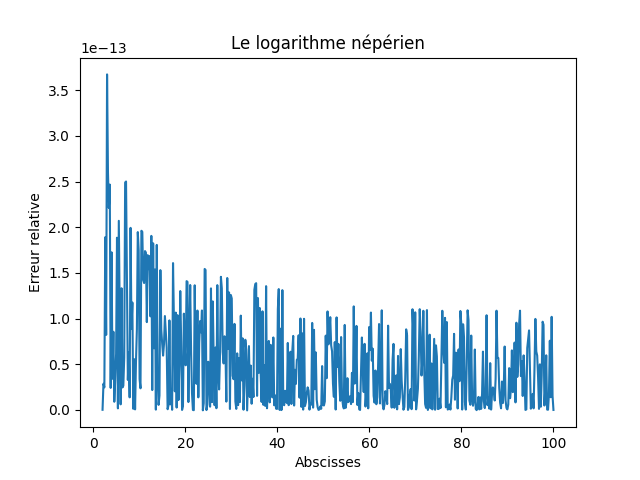
\includegraphics[width=1.1\linewidth]{images/er_ln.png}
         \caption{Représentation de l'erreur relative pour le calcul du logarithme népérien}\label{repr_err_rel_ln}
       \end{minipage}\hfill
       \begin{minipage}{0.48\textwidth}
         \centering
         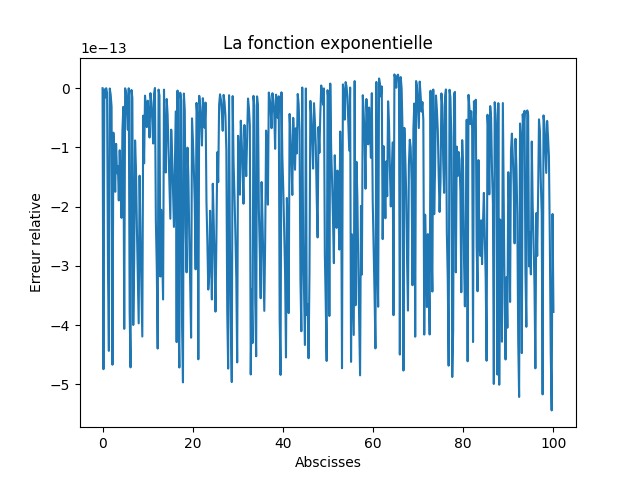
\includegraphics[width=1.1\linewidth]{images/er_exp.png}
         \caption{Représentation de l'erreur relative pour le calcul de l'exponentielle}\label{repr_err_rel_exp}
       \end{minipage}
    \end{figure}
    
    \begin{figure}[H]
       \begin{minipage}{0.48\textwidth}
         \centering
         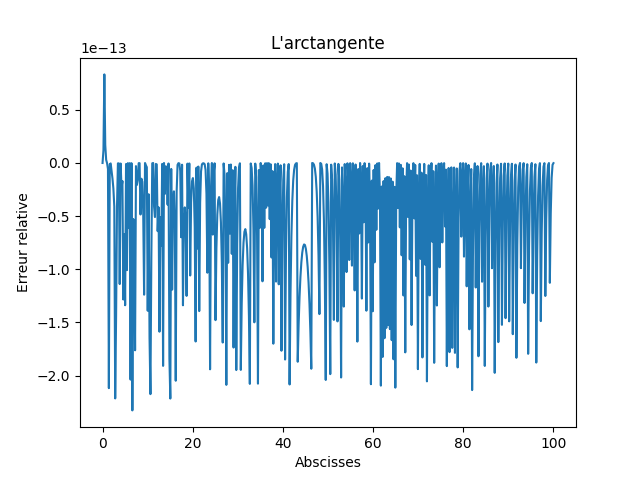
\includegraphics[width=1.1\linewidth]{images/er_atan.png}
         \caption{Représentation de l'erreur relative pour le calcul de l'arctangente}\label{repr_err_rel_arctan}
       \end{minipage}\hfill
       \begin{minipage}{0.48\textwidth}
         \centering
         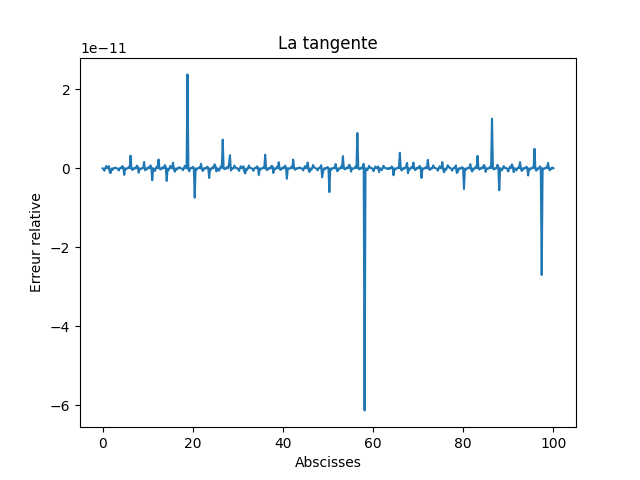
\includegraphics[width=1.1\linewidth]{images/er_tan.png}
         \caption{Représentation de l'erreur relative pour le calcul de la tangente}\label{repr_err_rel_tan}
       \end{minipage}
    \end{figure}
    
    \vspace{1em}
    \item
        \begin{enumerate}
            \item 
            Le premier problème traite l'évaluation des polynômes de degré 3 au moins. Ces derniers peuvent être évalués en moins de n multiplications. Soit $P \in \mathbb{R}_n[X]$ avec $n > 3$.
            \\Pour $n = 4$, P est naturellement de la forme: 
            \\$P(x) = a + b*x + c*x*x + d*x*x*x + e*x*x*x*x$ avec $(a,b,c,d,e) \in \mathbb{R}^5$ et $e \ne 0$
            \\En décomposant P en la somme d'un produit de deux polynômes de degré 2 et d'un réel tel que:
            \\$P(x) = [(A*x + B)^2 + A*x + C] * [(A*x + B)^2 + D] + E$
            où A,B,C,D,E sont des réels précalculés par: 
            \\$A=e^{(1/4)}$
            \\$B=(d-A^3)/(4A^3)$
            \\$D=3B^2+8B^3+(bA-2cB)/A^2$
            \\$C=(c/A)^2-2B-6B^2-D$
            \\$E=a-B^4-B^2(C+D)-CD$
            \\On passe de 10 multiplications à 3 et de 4 additions à 5. Comme les additions sont des opérations plus simples et moins complexes que les multiplications, on peut améliorer la méthode de calcul des polynômes en utilisant cette forme de décomposition.
            \item 
            D'une manière similaire, le deuxième problème traite la multiplication de deux nombres complexes.
            \\Soit $(x,y) \in \mathbb{C}^2$ $\exists!(a,b,c,d) \in \mathbb{R}^4$ tel que $x=a+ib$ et $y=c+id$
            \\On a donc $x*y=(ac-bd)+i(bc+ad)$ \textit{(E)}
            \\On peut réduire le nombre de multiplications en calculant le produit de la façon suivante:
            \\$x*y=(ac-bd)+i[(a+b)(c+d)-ac-bd]$ \textit{(F)}
            \\\textit{(E)} et \textit{(F)} sont bien évidemment équivalentes, mais on a réduit le nombre de multiplications de 4 à 3. Comme la multiplication est une opération lente sur certaines machines, le calcul devient plus performant.
            \item
            Le troisième problème concerne le module d'un nombre complexe.
            Soit $x \in \mathbb{C}$ tel que $x=a+ib$ avec $(a,b) \in \mathbb{R}^2$. Son module est défini par: $|x|=\sqrt{a^2+b^2}$. Si a ou b est aussi grand que la racine carrée du plus grand nombre représentable sur machine, on risque d'obtenir un overflow malgré que le module soit représentable. Pour éviter cela, on peut calculer le module d'un nombre complexe de la façon suivante:
            \\Si $|a|>=|b|$ alors $|a+ib|=|a|\sqrt{1+(b/a)^2}$, sinon $|a+ib|=|b|\sqrt{1+(a/b)^2}$ 
        \end{enumerate}
\end{enumerate}




\section{Conclusion}
    Ce projet nous a permis de comprendre les conséquences de la représentation limitée  en précision des nombres dans les machines, et également dans quels cas ces imprécisions sont à prendre en compte. Dans la seconde partie du projet, nous avons vu que dans les cas où ces imprécisions dérangent il est possible de les contenir en utilisant des algorithmes astucieux, l'algorithme de CORDIC dans notre cas.
    Globalement ce projet fut une réussite tant par l'entente de notre équipe, que par les résultats trouvés.
    Une suite intéressante à ce projet serait de voir les effets de ces imprécisions sur des cas concrets (simulation physique, financières, ML, ...), voir les cas où elles deviennent gênantes et s'intéresser à leur réduction par différentes techniques.


\end{document}

